\subsection{GUI}\label{subsec:gui}
Die Funktionen, welche von Terasic für die Gestaltung des GUI zur Verfügung gestellt werden, sind für unser Projekt zu ineffizient. Um einen Text anzuzeigen, verwendet Terasic eine Funktion, die ein Alpha Blending an den Rändern der Buchstaben durchführt. Dabei wird die Schriftfarbe mit der Hintergrundfarbe gemischt. Dieser Prozess nimmt viel Zeit in Anspruch und hat wenig Nutzen. Wodurch bei jedem neuen Zeichnen eines Texts zugeschaut werden konnte, wie die Pixel gezeichnet wurden. Dies ist für unser Projekt unbrauchbar. Zudem war eine ansprechendere Schriftart nötig. Daher realisierten wir eine eigene Funktion, welche Texte zeichnet. Diese ist im Modul \textbf{simple\_text.c} umgesetzt.
\newpage
\paragraph{simple\_text.c}\mbox{}\\

Mit dem Open Source Tool \textit{The Dot Factory} liess sich eine Bitmap für die Schrifftart Arial generieren, welche 22 Punkte gross gewählt ist. Das Tool generiert zwei Arrays. Im Bitmap Array sind die Buchstaben in einer Bitmap gespeichert. Das Descriptor Array enthält Informationen über die Breite jedes Characters und den Offset in der Character Bitmap. Um den Offset eines Buchstabens zu bestimmen, wird der Character minus des ersten Characters in der Bitmap gerechnet. Dies ergibt den Index für das Descriptor Array, in welchem der Offset für die Bitmap gespeichert ist. In Abbildung \ref{img:bitmap} ist dieser Prozess veranschaulicht. In diesem Beispiel besteht die Bitmap aus den Buchstaben a, b und c. Für den Buchstaben b wird der Offset 1 ausgerechnet. Im Descriptor Arrey ist auf Position 1 die Breite 5 gespeichert und der Offset 10 für die Bitmap. Mit diesen Informationen kann die Funktion \textit{print\_string(x,y,color,font,font\_descriptor,string)} einen Text String zeichnen. Dabei werden nur die Pixel gezeichnet, welche in der Bitmap auf 1 gesetzt sind.

\begin{figure}[h]
	\centering
	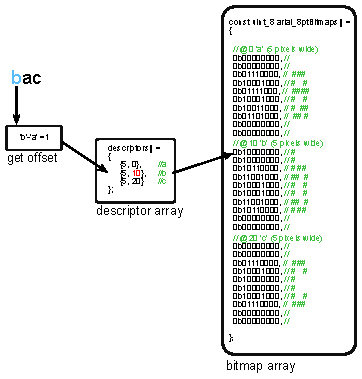
\includegraphics[width=0.8\textwidth]{the_dot_factory.pdf}
	\caption{Bitmap und Discriptor Array.}
	\label{img:bitmap}
\end{figure}

\newpage
\paragraph{gui.c} \mbox{}\\

In diesem Modul sind mit der Funktion \textit{print\_string(x,y,color,font,font\_descriptor,string)} aus dem Modul  \textit{simple\_text.c} und der Funktion \textit{LCD\_DrawRect(xs,ys,xe,ye,color)} aus dem Modul \textit{LT24\_controller.c} die einzelnen Menüs dargestellt. 